% ============================================================
%  Robot-Whisper —— 学术汇报 PPT(metropolis 主题 · TEAI 品牌蓝)
%  编译:latexmk -pdf main.tex   (pdflatex + CJKutf8 + Arphic gbsn)
% ============================================================
\documentclass[aspectratio=169,10pt]{beamer}
\usepackage{CJKutf8}
\usepackage{graphicx}
\usepackage{booktabs}
\renewcommand{\arraystretch}{1.15}
\usepackage{array}
\usepackage{amsmath,amssymb}
\usepackage{tikz}
\usepackage{qrcode}
\usetikzlibrary{arrows.meta,positioning}

\AtBeginDocument{\begin{CJK*}{UTF8}{gbsn}}
\AtEndDocument{\clearpage\end{CJK*}}

\usetheme[progressbar=frametitle,numbering=fraction,block=fill]{metropolis}

\definecolor{teai}{HTML}{1B5AD7}
\definecolor{teaidk}{HTML}{123C8F}
\definecolor{accent}{HTML}{B8860B}
\definecolor{alertc}{HTML}{AC372B}
\definecolor{okc}{HTML}{0C6E61}
\definecolor{mute}{HTML}{6E6757}
\definecolor{lightbg}{HTML}{F2F5FC}

\setbeamercolor{normal text}{fg=black!88,bg=white}
\setbeamercolor{alerted text}{fg=alertc}
\setbeamercolor{example text}{fg=okc}
\setbeamercolor{frametitle}{fg=white,bg=teai}
\setbeamercolor{progress bar}{fg=accent,bg=teai!25}
\setbeamercolor{title separator}{fg=accent}
\setbeamercolor{block title}{fg=white,bg=teai}
\setbeamercolor{block body}{bg=lightbg}
\setbeamercolor{palette primary}{fg=white,bg=teaidk}
\setbeamercolor{structure}{fg=teai}
\setbeamerfont{frametitle}{size=\large,series=\bfseries}
\setbeamertemplate{frametitle}{%
  \nointerlineskip\begin{beamercolorbox}[wd=\paperwidth,sep=0pt,leftskip=1.2em,rightskip=1em]{frametitle}%
  \vskip1.1ex\usebeamerfont{frametitle}\strut\insertframetitle\strut\vskip0.9ex%
  \end{beamercolorbox}}
\metroset{titleformat=regular,sectionpage=progressbar}
\linespread{1.15}\selectfont
\tolerance=2000 \emergencystretch=3em \hbadness=10000
\let\origCJKtilde\relax
\setbeamertemplate{frame footer}{\color{mute}Robot-Whisper\quad$\cdot$\quad 具身智能的内生异常警报}

\newcommand{\figbox}[1]{%
  \tikz[baseline=(I.center)]{\node[inner sep=0pt,draw=teai!45,line width=.7pt](I){\includegraphics[width=\linewidth]{#1}};}}
\newcommand{\hi}[1]{{\color{teai}\bfseries #1}}
\newcommand{\wi}[1]{{\color{accent}\bfseries #1}}
\newcommand{\bad}[1]{{\color{alertc}\bfseries #1}}
\newcommand{\ok}[1]{{\color{okc}\bfseries #1}}
\newcommand{\dimm}[1]{{\footnotesize\color{mute}#1}}
\newcommand{\warn}[1]{{\color{alertc}$\triangleright$~#1}}
\newcommand{\lead}[1]{{\large\color{teai}#1}\par\medskip}
\newcommand{\takeaway}[1]{%
  \begin{center}\begin{beamercolorbox}[wd=.94\textwidth,sep=6pt,rounded=true]{block body}%
  \centering #1\end{beamercolorbox}\end{center}}

\title{Neurons See the State the Tokens Don't}
\subtitle{具身智能的内生异常警报 —— 从神经元激活读出机器人的“卡住”}
\author{Robot-Whisper}
\institute{Institute of Trustworthy Embodied AI\quad$\cdot$\quad Fudan University}
\date{}
\titlegraphic{\hfill
\includegraphics[height=9mm]{assets/TEAI_logo.png}}

\begin{document}

\maketitle

\begin{frame}{提纲}
  \setbeamertemplate{section in toc}[sections numbered]
  \begin{columns}[T,onlytextwidth]
    \column{0.5\textwidth}\tableofcontents[hideallsubsections,sections={1-3}]
    \column{0.5\textwidth}\tableofcontents[hideallsubsections,sections={4-5}]
  \end{columns}
\end{frame}

\section{起点:从语言模型到具身}

%==================================================== P2a 两件旧事
\begin{frame}{起点:语言模型上的两个发现}
  \begin{columns}[T,onlytextwidth]
    \column{0.485\textwidth}
      {\color{teai}\bfseries ①\ NAD:神经元比 token 知道得多}\\[3pt]
      \parbox[c][2.55cm][c]{\linewidth}{\centering
      \begin{tikzpicture}[x=1cm,y=1cm,font=\scriptsize]
        \foreach \i in {0,...,5}{\foreach \j in {0,...,4}{\node[circle,draw=teai!45,inner sep=1.9pt] at (\i*0.4,\j*0.4) {};}}
        \foreach \i/\j in {0/1,1/3,2/0,3/2,4/1,5/3,1/0,3/4,5/0,2/2,0/4,4/4}{\node[circle,fill=teai,inner sep=1.9pt] at (\i*0.4,\j*0.4) {};}
        \node[text=mute] at (1.0,-0.5) {神经元活动 $\cdot$ 高维};
        \draw[-{Stealth},teai,thick] (2.5,0.8) -- (3.5,0.8) node[midway,above,text=teai]{投影};
        \node[text=alertc] at (3.0,0.5) {信息丢失};
        \foreach \k in {0,...,4}{\node[draw=mute!70,fill=lightbg,minimum width=0.46cm,minimum height=0.42cm,inner sep=0pt] at (3.85+\k*0.55,0.8) {};}
        \node[text=mute] at (4.95,-0.5) {token 序列 $\cdot$ 低维};
      \end{tikzpicture}}
      \vspace{-2pt}\footnotesize
      \begin{itemize}\setlength{\itemsep}{0pt}
        \item token 只是神经元活动的\hi{低维投影},投影会丢信息
        \item \textbf{不读一个字},凭激活模式就能挑出更可能对的答案
        \item 因而能在 CoT 的\hi{早期}就判断对错
      \end{itemize}
    \column{0.485\textwidth}
      {\color{alertc}\bfseries ②\ TAAR:长思维链会掉进 trap}\\[3pt]
      \parbox[c][2.55cm][c]{\linewidth}{\centering
      \begin{tikzpicture}[x=1cm,y=1cm,font=\scriptsize]
        \draw[thick,mute] plot[smooth,tension=0.8] coordinates {(0,1.8) (0.5,0.8) (1.1,0.2) (1.7,0.75) (2.3,1.4) (2.9,1.55) (3.5,1.05) (4.0,0.5) (4.5,0.75) (5.0,1.6)};
        \node[circle,fill=alertc!40,inner sep=2.2pt] at (0.38,1.05) {};
        \node[text=teai,font=\scriptsize\bfseries,anchor=east] at (0.27,1.05) {早期};
        \draw[teai,thick,dashed,-{Stealth}] (0.5,1.15) .. controls (1.5,2.2) and (3.0,2.2) .. (3.9,0.8);
        \node[text=teai,anchor=west] at (2.55,2.05) {早期:一次 resample 就跳出};
        \draw[alertc,-{Stealth}] (0.55,0.72) .. controls (0.75,0.42) .. (0.98,0.3);
        \node[text=alertc,anchor=east] at (0.92,0.22) {越想越深};
        \node[circle,fill=alertc,inner sep=2.4pt] at (1.1,0.32) {};
        \draw[alertc,dashed,-{Stealth}] (1.2,0.45) .. controls (1.4,1.0) and (1.7,0.95) .. (1.5,0.55);
        \draw[alertc,dashed,-{Stealth}] (1.2,0.45) .. controls (1.35,1.3) and (1.95,1.25) .. (1.68,0.78);
        \node[text=alertc] at (1.35,-0.1) {晚期:resample n 次都掉回来};
        \node[circle,fill=okc,inner sep=2.2pt] at (4.0,0.62) {};
        \node[text=okc] at (4.05,0.27) {正确答案};
      \end{tikzpicture}
      }
      \vspace{-2pt}\footnotesize
      \begin{itemize}\setlength{\itemsep}{0pt}
        \item 长 CoT 会掉进 \bad{Thinking Trap}(89\% 的失败):越想越深,根错不改
        \item 陷得越深越难出来:晚期 \textbf{resample 多次仍是错的}
        \item \hi{早期识别}到 trap,\wi{一次 resample} 就跳出错误盆地
      \end{itemize}
  \end{columns}
  \vspace{5pt}
  \begin{beamercolorbox}[wd=\textwidth,sep=4pt,rounded=true]{block body}\centering\footnotesize
    两件事合起来是一条链:\ \hi{内部信号比输出丰富}\ $\rightarrow$\ \bad{陷进 trap 出不来}\ $\rightarrow$\ \wi{早识别 + 重采样能逃出盆地}
  \end{beamercolorbox}
  \vspace{-2pt}
  {\tiny\color{mute}\setlength{\parskip}{0pt}
   ① Chen et al., \emph{Do LLMs Signal When They're Right? Evidence from Neuron Agreement} (NAD). arXiv:2510.26277 $\cdot$ ICML 2026 Spotlight\par
   ② Chen et al., \emph{Thinking Traps in Long Chain-of-Thought: A Measurable Study and Trap-Aware Adaptive Restart} (TAAR). arXiv:2601.11940 $\cdot$ Findings of ACL 2026\par}
\end{frame}

%==================================================== P2b 那么具身呢
\begin{frame}{那么具身呢?—— 把同一条链搬到 VLA 上}
  \footnotesize
  {\renewcommand{\arraystretch}{1.05}
  \begin{tabular}{@{}>{\leavevmode\color{mute}}p{1.4cm}>{\raggedright\arraybackslash}p{5.6cm}>{\raggedright\arraybackslash}p{6.4cm}@{}}
    \toprule
    & \textbf{\color{teai}LLM 推理(NAD / TAAR)} & \textbf{\color{teai}VLA 具身(本报告)} \\ \midrule
    轨迹 & reasoning trace(token 流) & interaction trajectory(动作流) \\
    内部信号 & 神经元激活(NAD) & 神经元激活 pattern(每步点亮哪些) \\
    trap & Thinking Trap:越想越深,根错不改 & 物理 trap:\textbf{动作在动,任务不前进} \\
    干预 & 早识别 + resample 一段 CoT & 早识别 + \textbf{冻结状态、换噪声重跑} rollout \\ \bottomrule
  \end{tabular}}
  \vspace{6pt}
  \begin{columns}[T,onlytextwidth]
    \column{0.47\textwidth}
      {\color{alertc}\bfseries 但具身更难}\\[2pt]
      \begin{itemize}\setlength{\itemsep}{1pt}
        \item 输出是\textbf{连续动作块},没有“对不对”可核对
        \item 每步接收新观测,错误会\textbf{改变物理世界}
        \item 策略\textbf{无记忆},连“我在重复”都不知道
      \end{itemize}
    \column{0.5\textwidth}
      {\color{teai}\bfseries 于是问同样的三个问题}\\[2pt]
      \begin{enumerate}\setlength{\itemsep}{1pt}
        \item 内部信号是否同样\textbf{比动作丰富}?\ \dimm{看得见吗}
        \item trap 是否在\textbf{神经元上留下痕迹}?\ \dimm{能报警吗}
        \item 重采样能否\textbf{跳出盆地}?\ \dimm{能救回吗}
      \end{enumerate}
  \end{columns}
  \vspace{4pt}
  \begin{beamercolorbox}[wd=\textwidth,sep=4pt,rounded=true]{block body}\footnotesize
    \textbf{预告答案:}\ok{能感知},神经元看得见 trap;\ \ok{可泛化},一套阈值跨任务不重调;\ \ok{能干预},报警步换条噪声就能救回。
  \end{beamercolorbox}
\end{frame}


%==================================================== §1 具身的 trap
\section{具身的 trap 长什么样}

%==================================================== P3 现象
\begin{frame}{具身的 trap:两条只差一条噪声的轨迹}
  \begin{columns}[T]
    \column{0.5\textwidth}\centering
      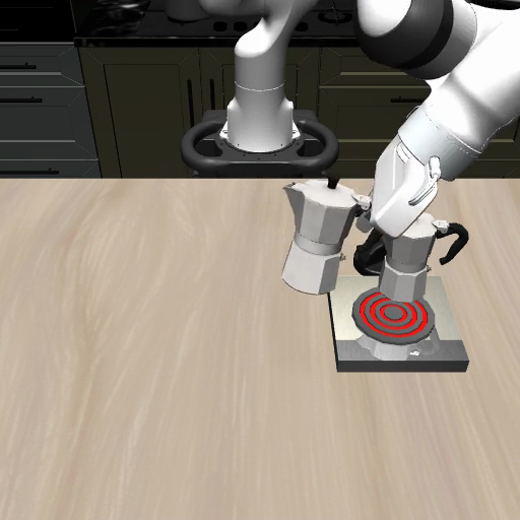
\includegraphics[width=\linewidth,height=3.1cm,keepaspectratio]{figs/succ.png}\\[3pt]
      {\color{teai}\bfseries $\checkmark$ 两只壶先后上炉}\\ \dimm{38 步 $\cdot$ 18.6 s}
    \column{0.5\textwidth}\centering
      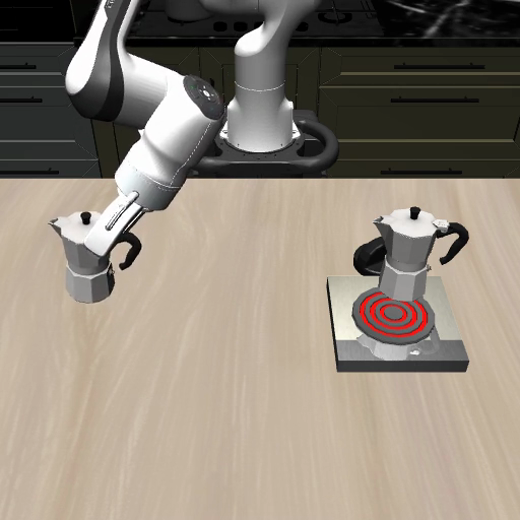
\includegraphics[width=\linewidth,height=3.1cm,keepaspectratio]{figs/fail.png}\\[3pt]
      {\color{alertc}\bfseries $\times$ 悬在第二只壶上方}\\ \dimm{52 步 $\cdot$ 26.0 s $\cdot$ 超时}
  \end{columns}
  \vfill
  \begin{center}\small
  同一个模拟器状态,唯一的区别是扩散头的\hi{一条采样噪声}。\\[3pt]
  右边掉进去之后 20 多步再没爬出来,直到超时 —— \bad{陷进去,出不来}。\\[3pt]
  \wi{而动作输出读起来一样正常:每一步照样吐出幅值正常的 10 帧。}
  \end{center}
  \vspace{-2pt}
  {\hfill\dimm{LLM 的 Thinking Trap $\leftrightarrow$ 这里}}
\end{frame}

%==================================================== P4 物理 trap
\begin{frame}{物理世界的 trap 长什么样}
  \begin{columns}[T]
    \column{0.62\textwidth}
      \figbox{figs/fig_trap.png}
    \column{0.36\textwidth}
      \small
      固定同一初始状态,只变采样噪声,跑 32 条:\\[2pt]
      \hi{14 成功} \quad / \quad \bad{18 超时}\\[8pt]
      纵轴是\textbf{累计变化量},不是到目标距离 ——\\
      \dimm{有的 trap 就停在目标旁边}\\[8pt]
      前半段同路:放好第一只壶(+13 cm),一起歇脚\\[6pt]
      \wi{分岔在第 30 步}:蓝色重新起跳;\\
      橙色\textbf{再也没涨过一厘米}
  \end{columns}
  \vfill
  \begin{center}\small 世界还在被改变,曲线就还在涨。\quad 掉进去的 18 条,\bad{没有一条自己爬出来} —— 这就是错误盆地。\end{center}
\end{frame}

%==================================================== P5 动作流是投影
\begin{frame}{不看模型内部也能检测 trap —— 但要付三笔代价}
  \vspace{1mm}
  \begin{columns}[T]
    \column{0.31\textwidth}
      {\color{accent}\bfseries 代价一\quad 仪器}\\[4pt]
      \small 要在外面建一条\textbf{反馈}:随时知道机械臂、物体在哪 —— 位姿真值、动捕、逐任务标定。\\[4pt]
      \dimm{仿真里免费,真机上多数场景拿不到。有了坐标确实最准(对卡住事件 $d{=}3.30$),但那是特权信息。}
    \column{0.31\textwidth}
      {\color{accent}\bfseries 代价二\quad 泛化}\\[4pt]
      \small trap 的物理样子\textbf{千差万别}:悬停、打转、拿起又放下;场景与任务也千差万别。规则写给一种,就漏掉别的。\\[4pt]
      \dimm{带量纲的阈值换任务就漂:动作幅值 100 点、坐标 24 点;两阶段任务全员误报。}
    \column{0.31\textwidth}
      {\color{accent}\bfseries 代价三\quad 滞后}\\[4pt]
      \small 靠\textbf{形状}判定(数圈、计时)得等一圈闭合,或等过自然停顿才敢报。\\[4pt]
      \dimm{成功轨迹放好第一只壶后自己也会歇十几步,第 30 步才再起跳;计时窗口要盖过这段,报警就滑到 q45 以后,而超时在 q52。}
  \end{columns}
  \vfill
  \takeaway{\small 能检测。但要\bad{仪器}、\bad{不泛化}、还\bad{慢半拍} —— 我们想要的是:不加硬件、一套规则到处用、不等一圈闭合。}
\end{frame}

%==================================================== §2 ①
\section{①② 神经元能看见并报出 trap 吗}

%==================================================== P6 神经元
\begin{frame}{神经元:pattern 与它的动力学}
  \begin{columns}[T]
    \column{0.55\textwidth}
      \figbox{figs/fig_heat.png}
    \column{0.43\textwidth}
      \small
      每个控制步,模型点亮一小撮神经元\\[6pt]
      \hi{激活 pattern 本身就能定向感知 trap}:\\
      受困后同一批神经元反复点亮成\textbf{水平条纹};顺利时不断更换\\[4pt]
      再加上对\hi{动力学}的理解,效果更好:\\
      读更迭的\textbf{快慢}而非具体是谁,一套阈值跨场景、跨任务\\[6pt]
      \takeaway{\wi{pattern 负责感知,动力学负责泛化}\\[3pt]{\footnotesize 警报只有一句话:换手速度比自己刚出发时慢,连续 3 步,就报。}}
  \end{columns}
  \vfill
  \dimm{图:同一初始状态的成功(蓝)与受困(橙)轨迹;上排浅层、下排深层;金线为 trap 起点 t30。\textbf{越深的层,条纹越清楚。}}
\end{frame}

%==================================================== P9 结果
\begin{frame}{结果:抓住八成失败}
  \begin{center}
  \begin{tabular}{@{}c@{\hskip 1.4cm}c@{\hskip 1.4cm}c@{}}
    {\Huge\color{teai}\bfseries 81.2\%} & {\Huge\color{accent}\bfseries +19.7} & {\Huge\color{teai}\bfseries 80\%}\\[2pt]
    \dimm{在线判对 $\cdot$ 864 条 rollout} & \dimm{高出多数类基线(61.5\%)} & \dimm{失败召回 $\cdot$ 误报 17\%}\\
  \end{tabular}
  \end{center}
  \vspace{2pt}
  \begin{columns}[T]
    \column{0.47\textwidth}\centering
      \begin{tikzpicture}[x=0.021cm,y=1cm,font=\scriptsize]
        \fill[alertc] (0,1.15) rectangle (184,2.0);
        \fill[alertc!30] (184,1.15) rectangle (235,2.0);
        \node[white,font=\scriptsize\bfseries] at (92,1.575) {报警 $\cdot$ 抓住 184};
        \node[alertc,font=\scriptsize\bfseries] at (209.5,1.575) {漏 51};
        \node[left,text=mute] at (-4,1.575) {失败 235};
        \fill[teai] (0,0) rectangle (98,0.85);
        \fill[accent] (98,0) rectangle (117,0.85);
        \node[white,font=\scriptsize\bfseries] at (49,0.425) {安静 $\cdot$ 判对 98};
        \node[right,text=accent!85!black,font=\scriptsize\bfseries] at (118,0.425) {误报 19};
        \node[left,text=mute] at (-4,0.425) {成功 117};
        \draw[mute] (0,-0.12) -- (235,-0.12);
        \foreach \x in {0,50,100,150,200} {\draw[mute] (\x,-0.12) -- (\x,-0.22) node[below,text=mute,inner sep=1pt]{\x};}
      \end{tikzpicture}\\[2pt]
      \dimm{判决矩阵 $\cdot$ 存档批次 352 条}
    \column{0.51\textwidth}\centering
      \begin{tikzpicture}[x=0.15cm,y=0.046cm,font=\scriptsize]
        \foreach \l/\f/\t in {18/10/10,20/9/16,22/19/20,24/15/16,26/31/31,28/33/34,30/42/46,32/17/21,34/6/7,36/2/2}{
          \fill[alertc] (\l,0) rectangle (\l+2,\f);
          \fill[accent] (\l,\f) rectangle (\l+2,\t);
        }
        \draw[mute] (16,0) -- (54,0);
        \foreach \x in {20,30,40,50} {\draw[mute] (\x,0) -- (\x,-2) node[below,text=mute,inner sep=1pt]{q\x};}
        \draw[mute] (16,0) -- (16,48);
        \foreach \y in {0,20,40} {\draw[mute] (16,\y) -- (15.3,\y) node[left,text=mute,inner sep=1pt]{\y};}
        \draw[dashed,teai,thick] (28,0) -- (28,52) node[above,text=teai,font=\scriptsize\bfseries]{中位 q28};
        \draw[dashed,mute] (52,0) -- (52,52) node[above,text=mute]{超时 q52};
      \end{tikzpicture}\\[2pt]
      \dimm{{\color{alertc}$\blacksquare$} 失败上的报警 184\quad {\color{accent}$\blacksquare$} 慢成功上的误报 19}
  \end{columns}
  \vspace{5pt}
  \begin{center}\small 跨\textbf{不同任务、不同初始状态};不看画面、动作、任务标签。\ \dimm{四个常数事先冻结,之后没有再调。}\end{center}
\end{frame}

%==================================================== P8b ① 的答案
\begin{frame}{神经元怎么回应这三笔代价}
  \vspace{1mm}
  \begin{columns}[T]
    \column{0.31\textwidth}
      {\color{teai}\bfseries 回应一\quad 零硬件}\\[4pt]
      \small 信号来自模型\textbf{前向传播本身}:每一步点亮哪些神经元,推理时顺手就有。不加传感器,不要坐标,不看画面。
    \column{0.31\textwidth}
      {\color{teai}\bfseries 回应二\quad 特异性}\\[4pt]
      \small 世界里有千种卡法,模型里只有\textbf{一种}:环锁死,更新停转。停滞类塌到 $r{\approx}0.45$ 的不动点;打转类多数也减速,少数一直在动,是漏报来源(召回 80\%)。\\[4pt]
      \dimm{只读换手速度,不读身份(身份是场景指纹);无量纲,阈值搬 22 个任务只漂 8 点。}
    \column{0.31\textwidth}
      {\color{teai}\bfseries 回应三\quad 不等一圈}\\[4pt]
      \small 不需要看到 trap 的完整形状:连续 \textbf{3 步}(1.5 s)更新变慢就报。报警中位 q28,距超时还有一半路程;报警步换一条噪声,\hi{3/8} 救回。
  \end{columns}
  \vspace{2pt}
  \takeaway{\small 回答 ①:看得见 —— 而且是\hi{免硬件}、\hi{跨任务}、\hi{不等一圈}的那种看得见。}
\end{frame}


%==================================================== §5 ③
\section{③ 能救回吗:干预}

%==================================================== P13 急救
\begin{frame}{急救!!\quad 报警那一步,做一下干预}
  \begin{columns}[T]
    \column{0.5\textwidth}
      \figbox{figs/fig_rescue.png}
    \column{0.46\textwidth}\small
      q32 报警 $\rightarrow$ \textbf{冻结状态} $\rightarrow$ 只加一点干扰
      (大幅度改换采样噪声)$\rightarrow$ 继续。其余一切不动。\\[8pt]
      \begin{tabular}{@{}lr@{}}
        \toprule
        救回 & \hi{3 / 8} \\
        步数 & 52 步失败 $\rightarrow$ \hi{8 步完成} \\
        时长 & 26.0 s $\rightarrow$ \hi{3.9 s} \\ \bottomrule
      \end{tabular}
  \end{columns}
  \vspace{4pt}
  \dimm{TAAR 的做法是按陷得深浅调重启力度(轻则重采样,重则强重启);我们只试了一种扰动 —— “陷得越深,扰动越强”是自然的下一步。}
\end{frame}

%==================================================== §6 结论
\section{结论}

%==================================================== P14 结论
\begin{frame}{结论:回到那三个问题}
  \begin{enumerate}
    \item[\wi{①}] \textbf{看得见吗} —— 看得见:同场景内 AUC 0.80,而且\hi{免硬件}、\hi{一套阈值跨任务}(飘移 8 点 vs 100 点)、\hi{不等一圈闭合}\\[3pt]
    \item[\wi{②}] \textbf{能报警吗} —— 能:四个事先冻结的常数,864 条 rollout 判对 \hi{81.2\%},
          召回 80\%、误报 17\%\\[3pt]
    \item[\wi{③}] \textbf{能救回吗} —— 部分能:报警那一步换一条噪声,\hi{3/8} 救回,
          26.0 s 的失败变成 3.9 s 的成功
  \end{enumerate}
  \vfill
  \takeaway{具身与语言的差别,不在\textbf{能不能看见},在\bad{能不能提前}:神经元激活是观测的函数,不可能比世界更早知道。}
  \begin{center}{\small github.com/Cck123123/Robot-Whisper}\end{center}
\end{frame}

%==================================================== L1 限制
\begin{frame}{限制清单}
  \small
  \begin{enumerate}
    \item \textbf{跨任务迁移只有一个标定源}(object/t00);留一交叉尚未做
    \item \textbf{失败样本稀少}:HUB 成功率 92--98\%,仅 6 个任务有 $\ge$3 条失败
    \item \textbf{跨本体无数据}:同一台 Franka、同一 checkpoint;“换机器人会崩”是量纲推论
    \item \textbf{相位混杂}:固定 t 比较时成功组已走完 $\sim$80\%、失败组 $\sim$60\%,
          所有统计量都部分在读进度
    \item \textbf{重放不可逐位复现}:模拟器快照不完整,干预实验引用存档首轮
    \item \textbf{单任务场景下神经元信号无优势}:policy\_state 更强($d{=}3.30$ vs $0.67$)也更简单
  \end{enumerate}
  \vfill
  \takeaway{\dimm{协议:组内配对 AUC 按配对数合并;置换检验 1500--5000 次;\textbf{跨组池化一律不用}
    —— 池化会把 0.586 抬到 0.86,读的是场景难度。}}
\end{frame}

\appendix
\begin{frame}[standout]
  防御页\\[4pt]{\small\normalfont Q\&A 按需翻出}
\end{frame}

%==================================================== D1
\begin{frame}{D1\quad “用动作幅值不就行了?”}
  \small\vfill
  \begin{center}
  \begin{tabular}{@{}lcccc@{}}
    \toprule
    \textbf{检测器} & \textbf{t=20} & \textbf{t=25} & \textbf{t=30} & \textbf{t=35} \\ \midrule
    动作幅值        & 0.638 & 0.622 & \bad{0.832} & 0.748 \\
    \textbf{神经元激活} & 0.478 & \hi{0.685} & 0.801 & 0.742 \\
    末端位移        & 0.564 & 0.656 & 0.795 & 0.763 \\
    仿真状态        & \bad{0.688} & \bad{0.761} & 0.761 & 0.736 \\
    模型输入状态    & 0.493 & 0.572 & 0.740 & 0.775 \\ \bottomrule
  \end{tabular}
  \end{center}
  \vfill
  \begin{alertblock}{诚实回答}
    \centering 是的,动作幅值在 $t{=}30$ 上赢了。\quad 但它赢在哪里 —— 见 D2。
  \end{alertblock}
  \vfill
  \dimm{场景$\times$快照内分层配对 AUC,置换检验;跨组池化一律不用。}
\end{frame}

%==================================================== D2
\begin{frame}{D2\quad 它是进度计,不是卡住检测器}
  \small
  \begin{center}
  \begin{tabular}{@{}lccc@{}}
    \toprule
    \textbf{量} & \textbf{失败组(卡住前$\rightarrow$后)} & \textbf{成功组(开头$\rightarrow$末段)} & \textbf{对 trap 的 $d$} \\ \midrule
    \textbf{神经元激活} & \hi{$-12.6\%$} & $-1.9\%$ & \hi{0.67} \\
    动作幅值          & $-5.5\%$ & \bad{$+24.1\%$} & \bad{0.03} \\
    模型输入状态      & $-67.2\%$ & $-26.1\%$ & \wi{3.30} \\
    末端位移          & $-1.7\%$ & $+27.6\%$ & $-0.12$ \\ \bottomrule
  \end{tabular}
  \end{center}
  \vfill
  \takeaway{动作幅值的判别力\textbf{八成来自“成功组末段猛干”}($+24\%$),
    不是“失败组卡住”($-5.5\%$)。\\
    对 trap 事件本身的效应量只有 \bad{0.03} 个标准差。}
\end{frame}

%==================================================== D3
\begin{frame}{D3\quad 时效:各检测器的报警时刻}
  \small\vfill
  \begin{center}
  \begin{tabular}{@{}lcc@{}}
    \toprule
    \textbf{检测器} & \textbf{检出率} & \textbf{报警中位} \\ \midrule
    动作幅值        & \bad{89.8\%} & q29 \\
    仿真状态        & 85.5\% & \bad{q25} \\
    末端位移        & 76.2\% & q30 \\
    \textbf{神经元激活} & \bad{56.2\%} & \bad{q31} \\ \bottomrule
  \end{tabular}
  \end{center}
  \vfill
  \takeaway{{\large\bad{“更早 / 更强”这两句话不能说。}}}
  \vfill
  \dimm{等误报率 $\approx$15\%、等机会窗口 t<37。}
\end{frame}

%==================================================== D4
\begin{frame}{D4\quad 那神经元赢在哪:跨任务阈值迁移}
  \footnotesize
  在 object/t00 标定到 15\% 误报,阈值\textbf{原样}搬到其余 22 个任务:
  \begin{center}
  \begin{tabular}{@{}lcccl@{}}
    \toprule
    \textbf{检测器} & \textbf{误报飘移} & \textbf{搬家后误报} & \textbf{搬家后检出} & \textbf{判读} \\ \midrule
    \textbf{神经元激活} & \hi{8 点} & 0\% & \hi{69\%} & \hi{可用} \\
    模型输入状态      & 24 点 & 10\% & 100\% & 可用,误报翻倍 \\
    动作幅值          & \bad{100 点} & 2\% & 100\% & 一个任务全员误报 \\
    动作块变化        & 10 点 & 0\% & \bad{7\%} & \bad{伪稳定 —— 等于关了} \\ \bottomrule
  \end{tabular}
  \end{center}
  \vfill
  \begin{columns}[T]
    \column{0.52\textwidth}
      \textbf{动作幅值为什么会 100\%:}\\
      标定任务是单阶段抓取;goal/t03 是“开抽屉+放碗”两阶段 —— 开头 8 步慢速接近
      $\rightarrow$ 自归一基线偏低 $\rightarrow$ 后半程全部越线
    \column{0.44\textwidth}
      \takeaway{\wi{任务内最强(0.832)\\ + 跨任务最脆(100 点)\\ 同时成立。}}
  \end{columns}
\end{frame}

%==================================================== D5
\begin{frame}{D5\quad 神经元信号稳的原因:三重不变性}
  \small\vfill
  \begin{center}
  \begin{tabular}{@{}clp{4.6cm}c@{}}
    \toprule
    & \textbf{层} & \textbf{内容} & \textbf{谁有} \\ \midrule
    \textcircled{1} & 归一化不变 & 集合重叠 $\in[0,1]$,不是“多少米/多少弧度” & \hi{仅神经元} \\
    \textcircled{2} & 重编号不变 & $|\cap|/|\cup|$ 不认神经元编号 & \hi{仅神经元} \\
    \textcircled{3} & 自身基线归一 & 除以自己开头 8 步(扣掉 67\% 场景方差) & 所有检测器 \\ \bottomrule
  \end{tabular}
  \end{center}
  \vfill
  \takeaway{{\large 神经元信号换来的不是判别力,是 \wi{“一次标定,到处能用”}。}\\[3pt]
    \small 这个价值在单任务 benchmark 上完全看不见,只在多任务/多本体部署时兑现。}
\end{frame}

%==================================================== D6
\begin{frame}{D6\quad 残差化:在外部量之外还剩什么}
  \small
  \begin{columns}[T]
    \column{0.54\textwidth}
      \begin{tabular}{@{}lcc@{}}
        \toprule
        & \textbf{AUC} & \textbf{p} \\ \midrule
        神经元激活(原始) & 0.801 & $<$0.0001 \\
        神经元激活 $\perp$ 模型输入状态 & \hi{0.780} & $<$0.0001 \\
        神经元激活 $\perp$ 输入+动作+仿真 & \hi{0.619} & 0.046 \\
        模型输入状态 $\perp$ 神经元激活 & 0.688 & $<$0.0001 \\ \bottomrule
      \end{tabular}
    \column{0.42\textwidth}
      \textbf{相关(秩):}\\[3pt]
      神经元 vs 输入状态\quad \hi{$+0.208$}\\
      \dimm{几乎不共线}\\[3pt]
      神经元 vs 动作幅值\quad $+0.562$\\
      神经元 vs 仿真状态\quad $+0.667$
  \end{columns}
  \vfill
  \begin{center}\small
  神经元激活不是输入的线性影子,但与“世界在不在动”共线较多;\\
  扣掉全部外部量后还剩 \hi{0.619},刚过显著线。
  \end{center}
\end{frame}

%==================================================== D7
\begin{frame}{D7\quad “试过别的切法吗?” —— 全部关闭}
  \footnotesize
  \begin{center}
  \begin{tabular}{@{}llc@{}}
    \toprule
    \textbf{方向} & \textbf{规模} & \textbf{结果} \\ \midrule
    组织方式暴力搜索 & 646 种 & 残差后全塌 \\
    聚合方式暴力搜索 & 13{,}494 种 & 时间聚合值 0.109 AUC,信号选择 $\le$2.5 点 \\
    马尔可夫 / MDP & 390 格 & 激活序列的链里没有 trap 集 \\
    卡尔曼 / SSM & --- & 0.69--0.71,输给基线 0.799 \\
    AR(2) 阻尼比 $\zeta$ & --- & 场景内 0.40--0.49 \\
    14 项峰值特征 & --- & 全零;唯一 $p<0.05$ 者复现符号翻转 \\
    9 项峰差比(TPR 族) & --- & 全零 \\
    token 之间的分歧 & --- & 0.472--0.543;效率靶子 $\rho=+0.001$ \\ \bottomrule
  \end{tabular}
  \end{center}
  \vfill
  \begin{columns}[T]
    \column{0.48\textwidth}
      \textbf{峰值族为什么必然失败:}\\
      连续摆幅比 $D_2/D_1$ 中位 \bad{1.053}(不衰减),与白噪声分布重合(AUC 0.480)。
      \textbf{没有瞬态,峰值法的前提不存在。}
    \column{0.48\textwidth}
      \textbf{核心解释:}\\
      chunk 间变化率是\hi{单一共享因子} —— 后块层与基线相关 0.95--0.97。
      \textbf{这个张量在“变化率”读法下只有一个自由度。}
  \end{columns}
\end{frame}

%==================================================== D8 口径修正
\begin{frame}{D8\quad 口径修正:blog 里三句话,这里怎么说}
  \small
  \begin{tabular}{@{}>{\raggedright\arraybackslash}p{3.7cm}>{\raggedright\arraybackslash}p{3.7cm}>{\raggedright\arraybackslash}p{5.9cm}@{}}
    \toprule
    \textbf{blog 原句} & \textbf{实测} & \textbf{这里的说法} \\ \midrule
    动作流分不出“干活”与“打转” & 动作幅值 t=30 AUC 0.832 & 动作侧\textbf{能}分成败,但读的是任务阶段;对 trap 事件效应量 0.03 \\[4pt]
    卡住 $\rightarrow$ 观测不变 $\rightarrow$ 输入不变 & 47 维仿真状态中 19 维仍在变;末端位移保留 99\% & \textbf{任务相关分量}停止更新 —— 世界没停,是任务停了 \\[4pt]
    同样的神经元反复点亮,思考冻结 & 持久点亮的神经元只是少数 & 换手速度\textbf{降三分之一}($\bar d$ 0.72 $\rightarrow$ 0.63),不是冻结 \\ \bottomrule
  \end{tabular}
  \vfill
  \takeaway{\small 三处都主动改口径。对撞表放在这里,是把弱点变成可信度。}
\end{frame}

%==================================================== D9 零提前量(原 D8)
\begin{frame}{D9\quad 零提前量,而且有因果解释}
  \small
  \begin{columns}[T]
    \column{0.46\textwidth}
      \begin{tabular}{@{}lccc@{}}
        \toprule
        \textbf{窗口} & \textbf{占失败段} & \textbf{AUC} & \textbf{p} \\ \midrule
        前 16 步 & 32\% & 0.537 & 0.48 \\
        前 20 步 & 40\% & 0.519 & 0.73 \\
        前 24 步 & 48\% & 0.461 & 0.46 \\
        \textbf{前 30 步} & \textbf{60\%} & \bad{0.236} & \bad{$<$0.0001} \\ \bottomrule
      \end{tabular}\\[6pt]
      \dimm{信号在 q24$\rightarrow$q30 之间出现,而 trap onset 正在 q30。}
    \column{0.5\textwidth}
      \takeaway{\scriptsize
        世界:\ 可改变 --- $\times$ 不可改变\\
        观测:\ 在变\ \ \ --- $\times$ 不变\\
        神经元:\ 在换\ \ --- $\times$ 更新减慢\\[3pt]
        \bad{三者同时翻转。}神经元激活是观测的函数\\
        $\rightarrow$ 不可能比世界更早知道。}
      \textbf{模型对自己卡住毫无觉察:}\\
      \begin{tabular}{@{}lr@{}}
        激活熵(信心) & \bad{$-0.04\%$} \\
        token 之间的分歧 & $-0.5\%$ \\
        被点亮神经元的概率质量 & $+1.4\%$ \\
      \end{tabular}
  \end{columns}
\end{frame}

%==================================================== D10 bad case(原 误报是什么)
\begin{frame}{D10\quad Bad case:被误报的成功是什么样}
  \begin{columns}[T]
    \column{0.52\textwidth}
      \figbox{figs/fig_slow.png}
    \column{0.44\textwidth}\small
      被误报的成功中位 \wi{41 步},\\
      安静的成功中位 \hi{37 步}\\[6pt]
      它们确实\textbf{更慢} —— 减速、擦着不动点的引力边缘,又自己爬回巡航区\\[10pt]
      \takeaway{警报读作 \wi{“正在下坠”}\\ 而不是“必然坠毁”}
      \dimm{这也是急救实验采用的读法}\\[6pt]
      \dimm{阈值附近误报率随 $\theta$ 平滑变化,工作点不在断崖上;常数微调,结论不变。}
  \end{columns}
\end{frame}

\begin{frame}{谢谢!\quad 扫码了解更多}
  \vspace{2mm}
  \begin{columns}[T]
    \column{0.33\textwidth}\centering
      \vspace{5mm}\qrcode[height=3.6cm]{https://cckfdu.com/demo/robot-whisper/en}\\[10pt]
      {\small\bfseries 项目网页}\\ \dimm{cckfdu.com/demo/robot-whisper}
    \column{0.33\textwidth}\centering
      
\includegraphics[height=4.6cm]{figs/contact_wechat.jpg}\\[4pt]
      {\small\bfseries 微信交流群}
    \column{0.33\textwidth}\centering
      
\includegraphics[height=4.6cm]{figs/contact_qq.jpg}\\[4pt]
      {\small\bfseries QQ 交流群}
  \end{columns}
  \vfill
  \begin{center}\dimm{github.com/Cck123123/Robot-Whisper}\end{center}
\end{frame}

\end{document}
